\documentclass[UTF8,zihao=-4]{ctexart}
\usepackage[a4paper,margin=2.1cm]{geometry}
\usepackage{array}
\usepackage{longtable}
\usepackage{hyperref}
\usepackage{verbatim}
\usepackage{graphicx}
\usepackage{tikz}
\usetikzlibrary{arrows.meta,positioning,fit,calc,shapes.geometric}
\hypersetup{hidelinks}
\setlength{\parindent}{0pt}
\setlength{\parskip}{0.55em}
\renewcommand{\arraystretch}{1.22}
\setlength{\tabcolsep}{3pt}
\emergencystretch=4em
\sloppy
\title{00 前置导入复习讲义}
\author{}
\date{}
\begin{document}
\maketitle
\tableofcontents
\newpage


整理范围：

\begin{itemize}
\item \texttt{PPT/00-00-课程Overview.pdf}
\item \texttt{PPT/00-01-AI辅助编程入门.pdf}
\item \texttt{PPT/00-02-开发工具链与Git工作流.pdf}
\item \texttt{PPT/00-03-AI编程进阶与Agent时代.pdf}
\item \texttt{PPT/00-04-前端开发基础.pdf}
\item \texttt{PPT/00-05-Java Web后端开发.pdf}
\item \texttt{PPT/00-06-项目级VibeCoding.pdf}
\end{itemize}

交叉参考：

\begin{itemize}
\item \texttt{Exam/2020.pdf}：Web 分层体系结构题，要求体现浏览器前端 \texttt{html}、\texttt{css}、\texttt{js} 在客户端，逻辑层和数据层在服务器端，通过 HTTP 和 REST 风格 API 通信。
\item \texttt{Exam/2022.pdf}：出现 \texttt{doPost(HttpRequest rsq, HttpResponse resp) throws ServletException, IOException} 代码，要求从软件构造角度分析，并基于该方法做测试覆盖。
\item \texttt{Exam/2025.pdf}：回忆题写明“题干 AI 浓度较高”，体系结构题要求描述 SpringBoot 三层职责，写 \texttt{Service} 接口、\texttt{Repository} 方法、\texttt{Controller} 调用 \texttt{Service} 的依赖注入代码片段。
\item \texttt{Review/summary-重点.pdf}、\texttt{Review/Final\_Reference.pdf}、\texttt{Review/软工II复习提纲by孙泽嵩.pdf}、\texttt{Review/软件工程与计算II重点整理(完整版).pdf}：对应需求类型、安全性、用例粒度、分层风格、MVC 风格、体系结构设计过程等旧考纲内容。
\end{itemize}

说明：Exam 和 Review 中未检索到 \texttt{VibeCoding}、\texttt{MCP}、\texttt{Stitch}、\texttt{AI Studio}、\texttt{Claude Code}、\texttt{Prompt Engineering} 的旧题直接对应段落。这些内容按 00 课件整理；前后端、REST、Servlet、SpringBoot 三层、安全性等内容按 PPT + Exam + Review 合并整理。

\section{一、00 部分整体定位}

00 部分不是单纯的工具介绍，而是为整门课建立三条基础线：

\begin{enumerate}
\item AI 协作线：会使用 AI，更要会审查 AI。
\item 工具链线：从本地开发、版本管理、自动部署到调试。
\item 全栈技术线：前端、后端、数据库、安全认证和项目级联调。
\end{enumerate}

这部分复习时不要只背工具名称，要把它们放回软件工程框架中：

\begin{itemize}
\item AI 输出需要人工审查，对应“工程判断力”和“批判性审查力”。
\item Git、CI/CD、Vercel 对应版本追踪、自动化测试、自动化部署、快速回滚。
\item Web 前后端对应分层体系结构、MVC、REST API 和接口设计。
\item Spring Security、JWT、BCrypt、最小权限对应安全性质量属性。
\item VibeCoding 对应“需求表达、Spec、审查、调试、联调”的完整工程流程。
\end{itemize}

\section{二、7 个课件的主线}

{
\footnotesize
\begin{longtable}{|>{\raggedright\arraybackslash}p{0.30\textwidth}|>{\raggedright\arraybackslash}p{0.30\textwidth}|>{\raggedright\arraybackslash}p{0.30\textwidth}|}
\hline
\textbf{课件} & \textbf{主线} & \textbf{必会关键词} \\
\hline
\endfirsthead
\hline
\textbf{课件} & \textbf{主线} & \textbf{必会关键词} \\
\hline
\endhead
\texttt{00-00} 课程 Overview & AI 时代软件工程课程如何重构 & K-A-S-D、三轨重构、提示→生成→审查→优化、四主体评价 \\
\hline
\texttt{00-01} AI 辅助编程入门 & AI 编程工具能做什么、不能做什么 & Copilot、Cursor、通义灵码、Claude Code、六大能力、提示词四要素 \\
\hline
\texttt{00-02} 开发工具链与 Git 工作流 & 从代码到线上 & DevOps、Git 四区域、Git 六命令、GitHub PR、Vercel \\
\hline
\texttt{00-03} AI 编程进阶与 Agent 时代 & 项目级 AI、代码质量、Agent & Spec、Skill、Debug 流程、测试生成、AI Code Review \\
\hline
\texttt{00-04} 前端开发基础 & Web、Vue、Node.js & HTML/CSS/JavaScript、AJAX、DOM、MVVM、SFC、Express、CORS \\
\hline
\texttt{00-05} Java Web 后端开发 & RESTful API、持久化、安全认证 & HTTP、Tomcat、Servlet、REST、JSON、Spring Boot、MyBatis、Spring Security、JWT \\
\hline
\texttt{00-06} 项目级 VibeCoding & AI 驱动全栈开发实战 & Stitch、AI Studio、Claude Code、通义灵码、Expo Go、MCP chrome-devtools \\
\hline
\end{longtable}
}


\section{三、课程 Overview：AI 时代软件工程的总框架}

\subsection{1. 课程核心判断}

课件中的核心判断是：

\begin{quote}
\footnotesize
\begin{verbatim}
AI 时代学生最大的短板，不是“用不好 AI”，而是“不知道什么时候不能信 AI”。
\end{verbatim}
\end{quote}

答题时要强调：

\begin{itemize}
\item AI 可以生成初稿，但不能承担工程责任。
\item 人负责需求理解、边界判断、架构决策、质量审查、安全合规和最终决策。
\item 工程师的价值从“手写所有代码”转向“定义问题、约束输出、审查结果、处理模糊性”。
\end{itemize}

\subsection{2. 五类 AI 无法替代的高阶工程能力}

{
\footnotesize
\begin{longtable}{|>{\raggedright\arraybackslash}p{0.30\textwidth}|>{\raggedright\arraybackslash}p{0.30\textwidth}|>{\raggedright\arraybackslash}p{0.30\textwidth}|}
\hline
\textbf{能力} & \textbf{解释} & \textbf{AI 的局限} \\
\hline
\endfirsthead
\hline
\textbf{能力} & \textbf{解释} & \textbf{AI 的局限} \\
\hline
\endhead
工程判断力 & 复杂情境中的独立决策 & AI 缺乏业务上下文与领域常识 \\
\hline
批判性审查力 & 识别 AI 输出中的错误、歧义、遗漏 & AI 不能可靠审查自身输出 \\
\hline
全局整体观 & 跨需求、架构、代码、测试的一致性审视 & AI 上下文有限，容易局部正确、整体冲突 \\
\hline
沟通与协商 & 理解并协调利益相关者意图 & AI 不能替代人际信任与责任承担 \\
\hline
伦理责任意识 & 安全、合规、知识产权、社会影响把关 & AI 没有主观责任感 \\
\hline
\end{longtable}
}


\subsection{3. 三轨重构}

{
\footnotesize
\begin{longtable}{|>{\raggedright\arraybackslash}p{0.30\textwidth}|>{\raggedright\arraybackslash}p{0.30\textwidth}|>{\raggedright\arraybackslash}p{0.30\textwidth}|}
\hline
\textbf{区间} & \textbf{含义} & \textbf{复习重点} \\
\hline
\endfirsthead
\hline
\textbf{区间} & \textbf{含义} & \textbf{复习重点} \\
\hline
\endhead
压缩区 & AI 可辅助完成的操作性任务 & 代码骨架、文档格式化、初步需求抽取 \\
\hline
强化区 & 人类核心判断任务 & 需求冲突、系统边界、架构权衡、可测试性、安全审查 \\
\hline
新增区 & AI 时代特有能力 & 提示词工程、AI 输出审查、人机协作工作流 \\
\hline
\end{longtable}
}


常见答题句：

\begin{quote}
\footnotesize
\begin{verbatim}
AI 能提升生成效率，但需求冲突判断、架构权衡、安全合规和最终责任仍必须由工程师承担。
\end{verbatim}
\end{quote}

\subsection{4. 四步工程协作范式}

\begin{quote}
\footnotesize
\begin{verbatim}
提示 → 生成 → 审查 → 优化
\end{verbatim}
\end{quote}

{
\footnotesize
\begin{longtable}{|>{\raggedright\arraybackslash}p{0.30\textwidth}|>{\raggedright\arraybackslash}p{0.30\textwidth}|>{\raggedright\arraybackslash}p{0.30\textwidth}|}
\hline
\textbf{步骤} & \textbf{学生行为} & \textbf{考点} \\
\hline
\endfirsthead
\hline
\textbf{步骤} & \textbf{学生行为} & \textbf{考点} \\
\hline
\endhead
提示 & 结构化、约束化、角色化表达需求 & Prompt Engineering \\
\hline
生成 & AI 完成知识密集型初稿 & 理解能力边界 \\
\hline
审查 & 识别错误、歧义、遗漏、冲突 & 批判性工程判断 \\
\hline
优化 & 修订提示词和结果，迭代到规范 & 过程留痕和质量提升 \\
\hline
\end{longtable}
}


\subsection{5. K-A-S-D}

{
\footnotesize
\begin{longtable}{|>{\raggedright\arraybackslash}p{0.30\textwidth}|>{\raggedright\arraybackslash}p{0.30\textwidth}|>{\raggedright\arraybackslash}p{0.30\textwidth}|}
\hline
\textbf{维度} & \textbf{含义} & \textbf{课件中的重点} \\
\hline
\endfirsthead
\hline
\textbf{维度} & \textbf{含义} & \textbf{课件中的重点} \\
\hline
\endhead
K & 知识掌握 & 核心概念、规范与原理、前沿技术 \\
\hline
A & AI 协作与判断 & 提示词写作、AI 输出驾驭、批判审查、冲突识别、权衡决策、伦理把关 \\
\hline
S & 工程技能 & 文档编写、需求分析、代码产出、工具使用、代码质量、调试、版本管理 \\
\hline
D & 过程与态度 & 作业态度、时间管理、自主学习、团队协作 \\
\hline
\end{longtable}
}


课件写明 A 维度占比 40\%，是 AI 时代软件工程师核心竞争力的直接体现。

\section{四、AI 辅助编程与 Agent}

\subsection{1. AI 编程工具生态}

{
\footnotesize
\begin{longtable}{|>{\raggedright\arraybackslash}p{0.30\textwidth}|>{\raggedright\arraybackslash}p{0.30\textwidth}|>{\raggedright\arraybackslash}p{0.30\textwidth}|}
\hline
\textbf{工具} & \textbf{定位} & \textbf{核心优势} \\
\hline
\endfirsthead
\hline
\textbf{工具} & \textbf{定位} & \textbf{核心优势} \\
\hline
\endhead
GitHub Copilot & VS Code / IDEA 插件 & 代码补全、Inline Chat \\
\hline
Cursor & AI-First IDE & 对话驱动、多文件理解、项目级上下文 \\
\hline
通义灵码 & VS Code / IDEA 插件 & 国内网络友好、中文提示词、企业级场景 \\
\hline
ChatGPT / Claude & 通用 AI & 架构设计、解释、代码审查 \\
\hline
Claude Code & 终端 AI 编程 Agent & 读写文件、执行命令、管理 Git、完成多步任务 \\
\hline
\end{longtable}
}


\subsection{2. AI 编程六大核心能力}

{
\footnotesize
\begin{longtable}{|>{\raggedright\arraybackslash}p{0.45\textwidth}|>{\raggedright\arraybackslash}p{0.45\textwidth}|}
\hline
\textbf{能力} & \textbf{说明} \\
\hline
\endfirsthead
\hline
\textbf{能力} & \textbf{说明} \\
\hline
\endhead
代码生成 & 从自然语言描述生成代码 \\
\hline
代码解释 & 解释代码逻辑 \\
\hline
Bug 修复 & 定位并修复错误 \\
\hline
代码注释 & 生成文档注释 \\
\hline
测试生成 & 生成单元测试初稿 \\
\hline
代码重构 & 优化结构与质量 \\
\hline
\end{longtable}
}


答题重点：这些能力都要经过人工审查，不能等同于最终正确结果。

\subsection{3. 提示词四要素}

公式：

\begin{quote}
\footnotesize
\begin{verbatim}
角色 + 任务 + 约束 + 格式
\end{verbatim}
\end{quote}

差的提示词：

\begin{quote}
\footnotesize
\begin{verbatim}
帮我修 bug
\end{verbatim}
\end{quote}

好的提示词应包含：

\begin{itemize}
\item 角色：例如“熟悉 Java Spring Boot 的后端工程师”。
\item 任务：分析导致异常的根本原因。
\item 约束：只修改出错方法，不改其他代码。
\item 格式：给出修复后的完整方法代码，并用一句话解释原因。
\end{itemize}

\subsection{4. 10 个高频提示词模板}

{
\footnotesize
\begin{longtable}{|>{\raggedright\arraybackslash}p{0.30\textwidth}|>{\raggedright\arraybackslash}p{0.30\textwidth}|>{\raggedright\arraybackslash}p{0.30\textwidth}|}
\hline
\textbf{类型} & \textbf{模板} & \textbf{作用} \\
\hline
\endfirsthead
\hline
\textbf{类型} & \textbf{模板} & \textbf{作用} \\
\hline
\endhead
控制范围 & 仅修复此问题，不要修改其他代码 & 防止 AI 改动范围过大 \\
\hline
控制范围 & 请使用最小修改来解决此问题 & 保持现有代码风格 \\
\hline
换方案 & 换个思路来解决此问题 & 当前方案性能或逻辑不满意 \\
\hline
全局审查 & 仔细阅读全文，检查是否还有其他同类问题 & 防止只修局部 \\
\hline
项目理解 & 请为我梳理当前代码的整体逻辑 & 接手陌生项目 \\
\hline
可维护性 & 请提供详细的解释和行内代码注释 & 便于维护 \\
\hline
测试 & 生成测试用例来验证此更改，包含正常路径和异常路径 & 提升覆盖 \\
\hline
调试 & 增加详细的日志输出，方便追溯错误 & 定位问题 \\
\hline
简化 & 请简化代码逻辑，去除冗余部分 & 代码瘦身 \\
\hline
重构 & 优化代码结构，使其更加模块化，方便单元测试 & 改善设计 \\
\hline
\end{longtable}
}


\subsection{5. AI 辅助 Debug 的标准流程}

\begin{enumerate}
\item 提供完整上下文：错误堆栈、出错方法、调用方法。
\item 先让 AI 分析根因，不直接修改代码。
\item 确认分析后，用最小修改修复。
\item 生成测试用例验证修复：正常路径、边界条件、异常路径。
\end{enumerate}

答题句：

\begin{quote}
\footnotesize
\begin{verbatim}
直接让 AI “修复 
Bug”容易导致改动范围失控；应先要求根因分析，再要求最小修改，并用测试验证。
\end{verbatim}
\end{quote}

\subsection{6. AI Code Review 的作用与边界}

AI 适合检查：

\begin{itemize}
\item 语法和拼写错误。
\item 常见安全漏洞，例如 SQL 注入、XSS、权限验证缺失。
\item 局部性能问题，例如不必要循环、N+1 查询。
\item 可维护性问题，例如方法过长、命名不清晰。
\item 边界条件问题，例如空值、空列表、越界。
\end{itemize}

AI 不可靠的部分：

\begin{itemize}
\item 业务逻辑正确性。
\item 公司规范和隐式约束。
\item 需求合理性。
\item 架构决策。
\item 安全合规责任。
\end{itemize}

结论：

\begin{quote}
\footnotesize
\begin{verbatim}
AI Code Review 是人工审查的补充，不是替代。
\end{verbatim}
\end{quote}

\subsection{7. Agent、Spec、Skill}

Agent 的定义：

\begin{quote}
\footnotesize
\begin{verbatim}
能自主执行多步任务的 AI 系统。
\end{verbatim}
\end{quote}

传统 AI 工具：

\begin{quote}
\footnotesize
\begin{verbatim}
你输入 → AI 输出 → 你执行
\end{verbatim}
\end{quote}

AI Agent：

\begin{quote}
\footnotesize
\begin{verbatim}
你描述目标 → Agent 自主规划步骤 → Agent 调用工具执行 → Agent 
检查结果 → Agent 调整计划
\end{verbatim}
\end{quote}

Spec 的作用：

\begin{itemize}
\item Agent 执行的是你描述的需求，不是你脑子里的真实需求。
\item Spec 越精确，Agent 越可靠。
\item 这与需求工程中“系统级需求必须明确、可测试、可追踪”的原则一致。
\end{itemize}

Skill 的作用：

\begin{itemize}
\item 将可复用任务封装成技能模块。
\item 降低 Agent 在复杂项目中遗忘上下文的风险。
\item 例如“初始化新 API 接口”“审查这段代码”可以被固定为重复使用的工作流。
\end{itemize}

\section{五、DevOps、Git 与自动部署}

\subsection{1. DevOps}

DevOps：

\begin{quote}
\footnotesize
\begin{verbatim}
开发 Dev + 运维 Ops + 文化 / 工具 / 实践
\end{verbatim}
\end{quote}

核心流程：

\begin{quote}
\footnotesize
\begin{verbatim}
代码提交 → 自动测试 → 自动构建 → 自动部署 → 监控反馈 → 持续改进
\end{verbatim}
\end{quote}

答题角度：

\begin{itemize}
\item DevOps 打破开发和运维之间的壁垒。
\item 自动化流水线减少手工部署错误。
\item 分阶段发布、测试覆盖、自动回滚可以降低线上事故影响。
\end{itemize}

\subsection{2. Git 四个区域}

\begin{quote}
\footnotesize
\begin{verbatim}
工作区 Working Directory
  ↓ git add
暂存区 Index / Staging Area
  ↓ git commit
本地仓库 Local Repository
  ↓ git push
远程仓库 Remote Repository
  ↑ git pull / git fetch
\end{verbatim}
\end{quote}

\subsection{3. Git 六个常用命令}

{
\footnotesize
\begin{longtable}{|>{\raggedright\arraybackslash}p{0.45\textwidth}|>{\raggedright\arraybackslash}p{0.45\textwidth}|}
\hline
\textbf{命令} & \textbf{作用} \\
\hline
\endfirsthead
\hline
\textbf{命令} & \textbf{作用} \\
\hline
\endhead
\texttt{git clone} & 克隆远程仓库到本地 \\
\hline
\texttt{git add} & 添加到暂存区 \\
\hline
\texttt{git commit -m} & 提交到本地仓库 \\
\hline
\texttt{git push} & 推送到远程仓库 \\
\hline
\texttt{git pull} & 拉取并合并远程更新 \\
\hline
\texttt{git checkout -b} & 创建并切换分支 \\
\hline
\end{longtable}
}


其他必会命令：

\begin{itemize}
\item \texttt{git status}：查看工作区和暂存区状态。
\item \texttt{git log --oneline}：查看简洁提交历史。
\item \texttt{git diff}：查看未暂存修改。
\item \texttt{git reset HEAD filename.py}：从暂存区移出，不删除修改。
\item \texttt{git reset --soft HEAD\textasciitilde{}1}：撤销上一次 commit，保留修改在暂存区。
\item \texttt{git reset --hard}：永久丢弃修改，风险很高。
\end{itemize}

\subsection{4. GitHub 团队协作工作流}

\begin{quote}
\footnotesize
\begin{verbatim}
git clone
→ git checkout -b feature/xxx
→ 写代码
→ git add
→ git commit
→ git push origin feature/xxx
→ 创建 Pull Request
→ Code Review
→ 合并到 main
→ git pull origin main
\end{verbatim}
\end{quote}

关键习惯：

\begin{itemize}
\item 每次 commit 只做一件事。
\item commit message 写清楚。
\item 通过 PR 做代码审查。
\item main 分支需要保护。
\end{itemize}

\subsection{5. Vercel 自动部署}

基本流程：

\begin{quote}
\footnotesize
\begin{verbatim}
GitHub 仓库
→ Vercel 导入项目
→ git push 到 main
→ 自动构建和部署
→ 获得 HTTPS 链接
\end{verbatim}
\end{quote}

答题角度：

\begin{itemize}
\item 自动触发：每次 \texttt{git push} 到关联仓库。
\item 预览部署：每个 Pull Request 可生成独立预览链接。
\item 回滚：部署平台保留历史版本，便于恢复。
\end{itemize}

\section{六、前端开发基础}

\subsection{1. AJAX 与 Web 演进}

AJAX：

\begin{quote}
\footnotesize
\begin{verbatim}
Asynchronous JavaScript And XML
\end{verbatim}
\end{quote}

核心机制：

\begin{quote}
\footnotesize
\begin{verbatim}
用户操作
→ 浏览器后台发出 HTTP 请求
→ 服务器返回 JSON/XML 数据
→ JavaScript 更新局部 DOM
→ 页面不整体刷新
\end{verbatim}
\end{quote}

技术演进线：

\begin{quote}
\footnotesize
\begin{verbatim}
静态 HTML → 动态 JS → AJAX 异步 → 前端框架 → 组件化 → 全栈 
JS
\end{verbatim}
\end{quote}

AJAX 解决的问题：

\begin{itemize}
\item 避免整页刷新。
\item 提升交互流畅度。
\item 让 Web 应用接近桌面应用体验。
\end{itemize}

AJAX 引入的新复杂度：

\begin{itemize}
\item 状态管理。
\item SEO。
\item 浏览器前进/后退。
\item 前后端数据一致性。
\end{itemize}

\subsection{2. Web 前端三层架构}

{
\footnotesize
\begin{longtable}{|>{\raggedright\arraybackslash}p{0.30\textwidth}|>{\raggedright\arraybackslash}p{0.30\textwidth}|>{\raggedright\arraybackslash}p{0.30\textwidth}|}
\hline
\textbf{层} & \textbf{技术} & \textbf{职责} \\
\hline
\endfirsthead
\hline
\textbf{层} & \textbf{技术} & \textbf{职责} \\
\hline
\endhead
结构层 & HTML & 内容、结构、语义 \\
\hline
表现层 & CSS & 颜色、字体、布局、动画 \\
\hline
行为层 & JavaScript & DOM 操作、事件、异步通信、逻辑计算 \\
\hline
\end{longtable}
}


JavaScript 四大核心能力：

\begin{itemize}
\item DOM 操作。
\item 事件处理。
\item 异步通信：\texttt{fetch} / XHR。
\item 逻辑计算。
\end{itemize}

\subsection{3. DOM 与渲染}

浏览器渲染流水线：

\begin{quote}
\footnotesize
\begin{verbatim}
HTML → DOM 树
CSS → CSS 规则树
DOM + CSS → 渲染树
→ 布局
→ 绘制
→ 显示
\end{verbatim}
\end{quote}

JavaScript 修改 DOM 或样式会触发重新布局 Reflow 或重绘 Repaint。

\subsection{4. Vue.js}

Vue 的核心思想：

\begin{quote}
\footnotesize
\begin{verbatim}
数据驱动视图
\end{verbatim}
\end{quote}

MVVM：

{
\footnotesize
\begin{longtable}{|>{\raggedright\arraybackslash}p{0.45\textwidth}|>{\raggedright\arraybackslash}p{0.45\textwidth}|}
\hline
\textbf{部分} & \textbf{含义} \\
\hline
\endfirsthead
\hline
\textbf{部分} & \textbf{含义} \\
\hline
\endhead
Model & 数据 / API \\
\hline
View & HTML 模板 / 用户界面 \\
\hline
ViewModel & Vue 实例，负责数据绑定和响应式更新 \\
\hline
\end{longtable}
}


Vue 三大核心特性：

\begin{itemize}
\item 响应式数据：数据变化自动触发视图更新。
\item 组件化：UI 拆成可复用独立单元。
\item 渐进式：可逐步引入。
\end{itemize}

\subsection{5. SFC 单文件组件}

SFC 文件扩展名：

\begin{quote}
\footnotesize
\begin{verbatim}
.vue
\end{verbatim}
\end{quote}

三部分：

\begin{quote}
\footnotesize
\begin{verbatim}
<template> 视图层 </template>
<script setup> 逻辑层 </script>
<style scoped> 样式层 </style>
\end{verbatim}
\end{quote}

\texttt{scoped} 的作用：防止样式泄漏到其他组件。

\subsection{6. Vue 核心指令}

{
\footnotesize
\begin{longtable}{|>{\raggedright\arraybackslash}p{0.45\textwidth}|>{\raggedright\arraybackslash}p{0.45\textwidth}|}
\hline
\textbf{指令} & \textbf{用途} \\
\hline
\endfirsthead
\hline
\textbf{指令} & \textbf{用途} \\
\hline
\endhead
\texttt{v-bind} / \texttt{:} & 动态绑定属性 \\
\hline
\texttt{v-model} & 表单双向数据绑定 \\
\hline
\texttt{v-if} / \texttt{v-else} & 条件渲染，真正增删 DOM \\
\hline
\texttt{v-show} & 条件显示，切换 \texttt{display} \\
\hline
\texttt{v-for} & 列表渲染 \\
\hline
\texttt{v-on} / \texttt{@} & 事件监听 \\
\hline
\end{longtable}
}


口诀：

\begin{quote}
\footnotesize
\begin{verbatim}
bind 绑属性，model 双向，if 条件，for 列表，on 事件。
\end{verbatim}
\end{quote}

\subsection{7. Options API 与 Composition API}

{
\footnotesize
\begin{longtable}{|>{\raggedright\arraybackslash}p{0.30\textwidth}|>{\raggedright\arraybackslash}p{0.30\textwidth}|>{\raggedright\arraybackslash}p{0.30\textwidth}|}
\hline
\textbf{对比项} & \textbf{Options API} & \textbf{Composition API} \\
\hline
\endfirsthead
\hline
\textbf{对比项} & \textbf{Options API} & \textbf{Composition API} \\
\hline
\endhead
逻辑组织 & 按选项类型分散 & 按功能聚合 \\
\hline
复用方式 & Mixins & Composables \\
\hline
TypeScript & 支持有限 & 完整支持 \\
\hline
课件建议 & 简单组件 / 迁移项目 & 新项目 / 复杂逻辑 \\
\hline
\end{longtable}
}


Vue 3 官方推荐 Composition API + \texttt{<script setup>}。

\subsection{8. Node.js 与 Express}

Node.js：

\begin{quote}
\footnotesize
\begin{verbatim}
V8 引擎 + 事件循环 + 非阻塞 I/O
\end{verbatim}
\end{quote}

核心优势：

\begin{itemize}
\item 高并发。
\item 前后端同语言。
\item npm 生态丰富。
\end{itemize}

Express 核心：

\begin{quote}
\footnotesize
\begin{verbatim}
路由 + 中间件
\end{verbatim}
\end{quote}

示例职责：

\begin{itemize}
\item 路由决定“谁来处理”请求。
\item 中间件决定“怎么处理”请求，例如日志、鉴权、解析 body。
\end{itemize}

\subsection{9. 前后端联动}

课件中的典型结构：

\begin{quote}
\footnotesize
\begin{verbatim}
Vue(5173) ← axios → Node.js(8081)
\end{verbatim}
\end{quote}

关键点：

\begin{itemize}
\item 前端用 \texttt{axios.get(...)} 调后端 API。
\item 后端用 Express 提供 JSON 数据。
\item 当前端和后端端口不同，需要处理 CORS。
\end{itemize}

前端路由与后端路由：

{
\footnotesize
\begin{longtable}{|>{\raggedright\arraybackslash}p{0.23\textwidth}|>{\raggedright\arraybackslash}p{0.23\textwidth}|>{\raggedright\arraybackslash}p{0.23\textwidth}|>{\raggedright\arraybackslash}p{0.23\textwidth}|}
\hline
\textbf{类型} & \textbf{处理者} & \textbf{刷新方式} & \textbf{特点} \\
\hline
\endfirsthead
\hline
\textbf{类型} & \textbf{处理者} & \textbf{刷新方式} & \textbf{特点} \\
\hline
\endhead
前端路由 & Vue Router & 页面不刷新，只替换组件 & SPA 体验流畅，SEO 较难 \\
\hline
后端路由 & 服务器 & 整页刷新 & SEO 友好 \\
\hline
\end{longtable}
}


\section{七、Java Web 后端开发}

\subsection{1. TCP/IP 与 HTTP}

TCP/IP 四层：

{
\footnotesize
\begin{longtable}{|>{\raggedright\arraybackslash}p{0.30\textwidth}|>{\raggedright\arraybackslash}p{0.30\textwidth}|>{\raggedright\arraybackslash}p{0.30\textwidth}|}
\hline
\textbf{层} & \textbf{协议示例} & \textbf{作用} \\
\hline
\endfirsthead
\hline
\textbf{层} & \textbf{协议示例} & \textbf{作用} \\
\hline
\endhead
应用层 & HTTP、FTP、DNS & 为应用提供网络服务接口 \\
\hline
传输层 & TCP、UDP & 端到端传输、差错控制、流量控制 \\
\hline
网络层 & IP、ARP、ICMP & 路由选择、拥塞控制、网络互连 \\
\hline
网络接口层 & SLIP、PPP、IEEE802 & 物理可靠传输 \\
\hline
\end{longtable}
}


HTTP：

\begin{itemize}
\item 应用层协议。
\item 基于客户端-服务器模型。
\item 构建在 TCP 连接之上。
\item 具有无状态特性。
\end{itemize}

一次 HTTP 操作：

\begin{quote}
\footnotesize
\begin{verbatim}
URL 地址解析
→ DNS 解析
→ 封装 HTTP 请求
→ 建立 TCP 连接
→ 客户端发送请求
→ 服务器响应
→ 关闭连接或 Keep-Alive 保持
\end{verbatim}
\end{quote}

\subsection{2. URL、Request、Response}

URL 结构：

\begin{quote}
\footnotesize
\begin{verbatim}
http://blog.example.com:8080/users?gender=ma
le&page=1
协议   主机名             端口  路径   查询参数
\end{verbatim}
\end{quote}

HTTP Request：

\begin{quote}
\footnotesize
\begin{verbatim}
请求行：方法 + 路径 + HTTP 版本
Headers
Body
\end{verbatim}
\end{quote}

常用 HTTP 方法：

{
\footnotesize
\begin{longtable}{|>{\raggedright\arraybackslash}p{0.45\textwidth}|>{\raggedright\arraybackslash}p{0.45\textwidth}|}
\hline
\textbf{方法} & \textbf{用途} \\
\hline
\endfirsthead
\hline
\textbf{方法} & \textbf{用途} \\
\hline
\endhead
GET & 获取资源，不修改服务器数据 \\
\hline
POST & 新增或修改资源 \\
\hline
PUT & 更新资源，替换整体 \\
\hline
DELETE & 删除资源 \\
\hline
\end{longtable}
}


HTTP Response：

\begin{quote}
\footnotesize
\begin{verbatim}
状态行：HTTP 版本 + 状态码 + 状态消息
Headers
空行
Body
\end{verbatim}
\end{quote}

状态码：

{
\footnotesize
\begin{longtable}{|>{\raggedright\arraybackslash}p{0.30\textwidth}|>{\raggedright\arraybackslash}p{0.30\textwidth}|>{\raggedright\arraybackslash}p{0.30\textwidth}|}
\hline
\textbf{范围} & \textbf{含义} & \textbf{示例} \\
\hline
\endfirsthead
\hline
\textbf{范围} & \textbf{含义} & \textbf{示例} \\
\hline
\endhead
2xx & 成功 & 200 OK、201 Created \\
\hline
3xx & 重定向 & 301、304 \\
\hline
4xx & 客户端错误 & 400、401、404 \\
\hline
5xx & 服务器错误 & 500 \\
\hline
\end{longtable}
}


\subsection{3. Tomcat 与 Servlet}

Tomcat：

\begin{itemize}
\item Java Web 服务器。
\item Java Servlet 容器。
\item Spring Boot 内嵌 Tomcat。
\end{itemize}

Tomcat 核心职责：

\begin{itemize}
\item 管理 Servlet 生命周期。
\item URL 路由映射。
\item 请求/响应封装。
\end{itemize}

Servlet 生命周期：

\begin{quote}
\footnotesize
\begin{verbatim}
HTTP 请求到达
→ 容器加载 Servlet 类
→ init() 初始化，只执行一次
→ service() 每次请求触发
→ doGet() / doPost() 根据 HTTP 方法分发
→ destroy() 容器关闭时执行
\end{verbatim}
\end{quote}

Exam 对应：

\begin{itemize}
\item \texttt{Exam/2022.pdf} 中出现 \texttt{doPost(HttpRequest rsq, HttpResponse resp) throws ServletException, IOException} 代码。
\item 该题不是只考 Servlet 定义，还要求从软件构造角度分析代码优缺点，并围绕该方法计算圈复杂度、设计条件覆盖测试用例。
\end{itemize}

\subsection{4. REST 与 JSON}

REST：

\begin{quote}
\footnotesize
\begin{verbatim}
Representational State Transfer
\end{verbatim}
\end{quote}

核心特性：

\begin{itemize}
\item 无状态。
\item 统一接口。
\item 可扩展。
\item 分层系统。
\end{itemize}

REST API 设计：

\begin{quote}
\footnotesize
\begin{verbatim}
资源 + HTTP 方法
\end{verbatim}
\end{quote}

示例：

{
\footnotesize
\begin{longtable}{|>{\raggedright\arraybackslash}p{0.30\textwidth}|>{\raggedright\arraybackslash}p{0.30\textwidth}|>{\raggedright\arraybackslash}p{0.30\textwidth}|}
\hline
\textbf{操作} & \textbf{方法} & \textbf{URL} \\
\hline
\endfirsthead
\hline
\textbf{操作} & \textbf{方法} & \textbf{URL} \\
\hline
\endhead
获取全部商品 & GET & \texttt{/api/products} \\
\hline
获取单个商品 & GET & \texttt{/api/products/123} \\
\hline
新建商品 & POST & \texttt{/api/products} \\
\hline
更新商品 & PUT & \texttt{/api/products/123} \\
\hline
删除商品 & DELETE & \texttt{/api/products/123} \\
\hline
获取商品评论 & GET & \texttt{/api/products/123/reviews} \\
\hline
\end{longtable}
}


JSON：

\begin{itemize}
\item JavaScript Object Notation。
\item REST API 常用数据格式。
\item 数据类型包括 string、number、object、array、true/false、null。
\item MIME 类型是 \texttt{application/json}。
\item 文件扩展名是 \texttt{.json}。
\end{itemize}

\subsection{5. Spring Boot}

Spring Boot 核心优势：

{
\footnotesize
\begin{longtable}{|>{\raggedright\arraybackslash}p{0.45\textwidth}|>{\raggedright\arraybackslash}p{0.45\textwidth}|}
\hline
\textbf{特性} & \textbf{说明} \\
\hline
\endfirsthead
\hline
\textbf{特性} & \textbf{说明} \\
\hline
\endhead
约定优于配置 & 默认值覆盖多数场景，只配置例外情况 \\
\hline
自动配置 & 检测 classpath，自动装配组件 \\
\hline
Starter 依赖 & 一行引入一组依赖 \\
\hline
内嵌服务器 & fat JAR，\texttt{java -jar} 运行，自带 Tomcat \\
\hline
\end{longtable}
}


常用注解：

{
\footnotesize
\begin{longtable}{|>{\raggedright\arraybackslash}p{0.45\textwidth}|>{\raggedright\arraybackslash}p{0.45\textwidth}|}
\hline
\textbf{注解} & \textbf{作用} \\
\hline
\endfirsthead
\hline
\textbf{注解} & \textbf{作用} \\
\hline
\endhead
\texttt{@SpringBootApplication} & 启动入口，开启自动配置 \\
\hline
\texttt{@RestController} & 控制器，方法返回值自动序列化为 JSON \\
\hline
\texttt{@GetMapping("/path")} & 处理 HTTP GET 请求 \\
\hline
\texttt{@PostMapping("/path")} & 处理 HTTP POST 请求 \\
\hline
\texttt{@RequestBody} & 从请求体读取 JSON 并反序列化为对象 \\
\hline
\texttt{@PathVariable} & 从 URL 路径提取变量 \\
\hline
\texttt{@RequestParam} & 从 URL 查询字符串读取值 \\
\hline
\end{longtable}
}


关系：

\begin{quote}
\footnotesize
\begin{verbatim}
@RestController = @Controller + 
@ResponseBody
\end{verbatim}
\end{quote}

\subsection{6. MyBatis}

MyBatis 解决的问题：

\begin{itemize}
\item JDBC 连接管理繁琐。
\item 手动参数绑定繁琐。
\item 手动结果集映射繁琐。
\item 忘记关闭连接会导致连接泄漏。
\end{itemize}

MyBatis 自动处理：

\begin{itemize}
\item 连接管理。
\item 参数预编译绑定。
\item 结果集映射。
\item 异常转换。
\end{itemize}

安全重点：

\begin{quote}
\footnotesize
\begin{verbatim}
#{id} 是预编译参数，安全，防 SQL 注入。
${id} 是字符串拼接，危险，不能用于用户输入。
\end{verbatim}
\end{quote}

\subsection{7. Spring Boot / MyBatis 三层结构}

课件中的完整 MVC 分层结构：

\begin{quote}
\footnotesize
\begin{verbatim}
HTTP 请求
→ Controller：接收请求，参数校验，调用 Service
→ Service：业务逻辑，事务管理
→ Mapper：SQL 操作，返回实体对象
→ MySQL 数据库
\end{verbatim}
\end{quote}

Exam 对应：

\begin{itemize}
\item \texttt{Exam/2025.pdf} 回忆题写的是 \texttt{Controller}、\texttt{Service}、\texttt{Repository}。
\item \texttt{PPT/00-05} 课件写的是 \texttt{Controller}、\texttt{Service}、\texttt{Mapper}。
\item 答题时必须沿用题目给出的标识符。如果题目写 \texttt{Repository}，不要自行替换为 \texttt{Mapper}；如果题目写 \texttt{Mapper}，不要自行替换为 \texttt{Repository}。
\end{itemize}

三层职责答题模板：

\begin{quote}
\footnotesize
\begin{verbatim}
Controller 层负责接收 HTTP 请求、解析参数、进行基础校验、调用 
Service，并将结果组织为 HTTP/JSON 响应。
Service 层负责业务逻辑、业务规则编排、事务边界和对下层数据访问接口的调用。
Repository/Mapper 
层负责数据访问，封装数据库查询、插入、更新、删除操作，向上层返回实体对象或数据结果。
\end{verbatim}
\end{quote}

\subsection{8. Spring Security、JWT 与 BCrypt}

认证与授权：

{
\footnotesize
\begin{longtable}{|>{\raggedright\arraybackslash}p{0.23\textwidth}|>{\raggedright\arraybackslash}p{0.23\textwidth}|>{\raggedright\arraybackslash}p{0.23\textwidth}|>{\raggedright\arraybackslash}p{0.23\textwidth}|}
\hline
\textbf{概念} & \textbf{英文} & \textbf{回答的问题} & \textbf{示例} \\
\hline
\endfirsthead
\hline
\textbf{概念} & \textbf{英文} & \textbf{回答的问题} & \textbf{示例} \\
\hline
\endhead
认证 & Authentication / AuthN & 你是谁 & 用户名 + 密码登录 \\
\hline
授权 & Authorization / AuthZ & 你能做什么 & 管理员才能删除用户 \\
\hline
\end{longtable}
}


Spring Security 核心机制：

\begin{quote}
\footnotesize
\begin{verbatim}
过滤器链 Filter Chain
\end{verbatim}
\end{quote}

课件中的过滤器：

\begin{itemize}
\item \texttt{UsernamePasswordAuthenticationFilter}：处理表单登录。
\item \texttt{JwtAuthenticationFilter}：验证 Token，自定义。
\item \texttt{ExceptionTranslationFilter}：将异常转为 401 / 403 响应。
\item \texttt{FilterSecurityInterceptor}：最终权限检查。
\end{itemize}

JWT 流程：

\begin{quote}
\footnotesize
\begin{verbatim}
POST /api/auth/login
→ 服务端验证用户名和密码
→ 查数据库，BCrypt 比对
→ 生成 JWT Token
→ 客户端后续请求携带 Authorization: Bearer token
→ 服务端验证签名和过期时间
→ 通过后执行业务逻辑
\end{verbatim}
\end{quote}

JWT 三段：

\begin{quote}
\footnotesize
\begin{verbatim}
Header.Payload.Signature
\end{verbatim}
\end{quote}

重点：

\begin{itemize}
\item Header 记录签名算法。
\item Payload 记录用户信息，Base64 编码，不是加密。
\item Signature 用密钥签名，防篡改。
\item 不要把密码放入 Payload。
\item 密码存储应使用 \texttt{BCryptPasswordEncoder}，不能存明文密码。
\end{itemize}

\subsection{9. 安全性与 Review 对应}

Review 中对安全性的定义：

\begin{quote}
\footnotesize
\begin{verbatim}
软件阻止对其程序和数据进行未授权访问的能力，未授权访问包括有意访问和无意访问两类。
\end{verbatim}
\end{quote}

这与 00-05 的 Spring Security、JWT、BCrypt、最小权限原则直接对应。

Equifax 案例的三层原因：

\begin{itemize}
\item 依赖管理失控：没有自动漏洞扫描机制。
\item 认证授权缺失：内部子系统之间无身份验证。
\item 最小权限原则违反：数据库账号权限过大。
\end{itemize}

答题句：

\begin{quote}
\footnotesize
\begin{verbatim}
安全认证和访问授权不是孤立功能点，而是安全性质量属性在架构和实现层面的落地。
\end{verbatim}
\end{quote}

\section{八、项目级 VibeCoding}

\subsection{1. VibeCoding 定义}

VibeCoding 的核心思想：

\begin{quote}
\footnotesize
\begin{verbatim}
用自然语言描述意图，让 AI 完成实现。
\end{verbatim}
\end{quote}

但课件明确强调：

\begin{itemize}
\item VibeCoding 改变的是开发速度和交互方式。
\item 不变的是需求分析、架构设计、工程纪律、测试、安全审查和人的最终判断。
\end{itemize}

\subsection{2. 工具链}

{
\footnotesize
\begin{longtable}{|>{\raggedright\arraybackslash}p{0.30\textwidth}|>{\raggedright\arraybackslash}p{0.30\textwidth}|>{\raggedright\arraybackslash}p{0.30\textwidth}|}
\hline
\textbf{阶段} & \textbf{工具} & \textbf{作用} \\
\hline
\endfirsthead
\hline
\textbf{阶段} & \textbf{工具} & \textbf{作用} \\
\hline
\endhead
原型 & Google Stitch & 自然语言生成界面原型 \\
\hline
Web 前端 & Google AI Studio & 原型截图 + 技术栈描述，生成前端代码 \\
\hline
Web 后端 & Claude Code & 生成 Express 后端 API，读写项目文件，执行命令 \\
\hline
移动端 & 通义灵码 + Expo & 生成 React Native / Expo App \\
\hline
真机调试 & Expo Go & 手机扫码预览，热重载 \\
\hline
Web 自动调试 & MCP chrome-devtools & 读取 Console、Network、DOM，辅助定位前端问题 \\
\hline
\end{longtable}
}


\subsection{3. 完整工作流}

\begin{quote}
\footnotesize
\begin{verbatim}
需求
→ Stitch 原型
→ AI Studio 生成 Web 前端 / 通义灵码生成移动端
→ Claude Code 或通义灵码生成后端 API
→ 接入 AI API
→ Web 端用 MCP chrome-devtools 调试
→ 移动端用 Expo Go 调试
→ 前后端联调
→ 部署上线
\end{verbatim}
\end{quote}

\subsection{4. MCP}

MCP：

\begin{quote}
\footnotesize
\begin{verbatim}
Model Context Protocol
\end{verbatim}
\end{quote}

作用：

\begin{itemize}
\item 让 AI 与外部工具通信。
\item 让 AI 读取浏览器 Console、Network、DOM。
\item 让 AI 从“根据文字描述推断问题”变为“直接观察运行状态”。
\end{itemize}

\texttt{chrome-devtools} 调试流程：

\begin{quote}
\footnotesize
\begin{verbatim}
连接 Chrome DevTools
→ 读取 Console 错误
→ 读取 Network 请求
→ 检查 DOM 结构
→ 注入调试代码
→ 定位根因
→ 修改源代码
\end{verbatim}
\end{quote}

常见调试场景：

\begin{itemize}
\item 控制台报错。
\item 网络请求失败。
\item 页面样式异常。
\item 性能问题。
\item 内存泄漏。
\item 接口联调。
\end{itemize}

\subsection{5. VibeCoding 的工程判断}

VibeCoding 改变了：

\begin{itemize}
\item 原型验证速度。
\item 代码生成方式。
\item 人机协作方式。
\end{itemize}

VibeCoding 没有改变：

\begin{itemize}
\item 需求分析仍由人负责。
\item 系统设计和架构决策仍由人负责。
\item 安全性、性能、可维护性仍需人工审查。
\item 测试和部署不能省略。
\end{itemize}

答题句：

\begin{quote}
\footnotesize
\begin{verbatim}
VibeCoding 
降低了代码生成门槛，但提高了对需求表达、Spec、审查、测试和集成能力的要求。
\end{verbatim}
\end{quote}

\section{九、Exam / Review 对应表}

{
\footnotesize
\begin{longtable}{|>{\raggedright\arraybackslash}p{0.30\textwidth}|>{\raggedright\arraybackslash}p{0.30\textwidth}|>{\raggedright\arraybackslash}p{0.30\textwidth}|}
\hline
\textbf{来源} & \textbf{对应内容} & \textbf{复习用法} \\
\hline
\endfirsthead
\hline
\textbf{来源} & \textbf{对应内容} & \textbf{复习用法} \\
\hline
\endhead
\texttt{Exam/2020.pdf} & Web 框架分层体系结构：浏览器含前端 \texttt{html}、\texttt{css}、\texttt{js} 在客户端，逻辑层和数据层在服务器端，网络通信采用 HTTP，基于 REST 风格 API 接口 & 复习前后端分层、REST API、物理包图、展示层/逻辑层/数据层接口 \\
\hline
\texttt{Exam/2022.pdf} & \texttt{doPost}、\texttt{HttpRequest}、\texttt{HttpResponse}、\texttt{ServletException}、\texttt{IOException}；从软件构造角度分析代码，并做测试覆盖 & 复习 Servlet、HTTP 请求参数、代码可读性、异常路径、边界条件、测试覆盖 \\
\hline
\texttt{Exam/2025.pdf} & 题干 AI 浓度较高；SpringBoot 三层内容职责；\texttt{Service}、\texttt{Repository}、\texttt{Controller}、依赖注入；三层顺序图 & 复习 AI 审查意识、SpringBoot 三层职责、接口声明、依赖注入、层间调用 \\
\hline
\texttt{Review/Final\_Reference.pdf} & 需求类型：功能、性能、质量属性、对外接口、约束、数据需求 & 区分安全认证、网络通信、API、数据字段分别属于什么类型 \\
\hline
\texttt{Review/summary-重点.pdf} & 安全性定义；不要把登录、数据验证、连接数据库、网络传输当作独立用例 & 把 00-05 的认证、授权、SQL 注入防护放入质量属性和实现约束中 \\
\hline
\texttt{Review/summary-重点.pdf} & 分层风格、MVC 风格、体系结构设计过程 & 支撑 2020 和 2025 的 Web 分层、MVC、三层架构题 \\
\hline
\texttt{Review/软工II复习提纲by孙泽嵩.pdf}、\texttt{Review/软件工程与计算II重点整理(完整版).pdf} & MVC 典型实现：View：JSP、HTML；Controller：Servlet；Model：JavaBean & 对接 00-04 前端、00-05 Servlet 和 Spring Boot 的现代实现 \\
\hline
\end{longtable}
}


Review 高频补强：

\begin{itemize}
\item \texttt{Review/Final\_Reference.pdf} 把质量保障拆到需求、体系结构、详细设计、构造、测试阶段；00 中的 AI 生成代码也要落回这些质量活动，用评审、测试、质量度量和持续集成兜底。
\item \texttt{Review/summary-重点.pdf} 明确登录、安全性、数据验证、连接数据库、网络传输不能写成业务用例；00 中的认证、授权、REST、数据库访问都要按质量属性、对外接口、约束或实现机制回答。
\item \texttt{Review/summary-重点.pdf} 强调体系结构接口定义：先确定模块对外接口，再确定接口规范；00 中的 \texttt{Controller}、\texttt{Service}、\texttt{Repository} 代码题按这个顺序写。
\item \texttt{Exam/2020.pdf}、\texttt{Exam/2022.pdf}、\texttt{Exam/2025.pdf} 连续考分层包图、REST API、三层接口、依赖注入和顺序图；00 的 Web 基础要能直接服务这些题。
\end{itemize}

\section{十、常见答题模板}

\subsection{1. 为什么有了 AI 还要学编程基础？}

\begin{quote}
\footnotesize
\begin{verbatim}
AI 可以生成代码，但生成结果需要人审查。没有编程基础，就无法判断代码是否正确、安全、可
维护，也无法识别边界条件、并发安全和性能问题。提示词质量取决于对问题的理解深度，基础
越扎实，约束越明确，AI 输出越可控。
\end{verbatim}
\end{quote}

\subsection{2. 好提示词应包含什么？}

\begin{quote}
\footnotesize
\begin{verbatim}
好提示词应包含角色、任务、约束和格式。角色限定 AI 的专业视角，任务说明要完成什么，约
束控制修改范围和工程边界，格式规定输出形态，便于审查和落地。
\end{verbatim}
\end{quote}

\subsection{3. AI Code Review 能否替代人工 Code Review？}

\begin{quote}
\footnotesize
\begin{verbatim}
不能。AI 擅长发现语法错误、常见安全漏洞、局部性能问题和可维护性问题，但不了解业务逻辑
、组织规范、隐式约束和需求合理性。AI Code Review 
是人工审查的补充，不是替代。
\end{verbatim}
\end{quote}

\subsection{4. DevOps 的核心价值是什么？}

\begin{quote}
\footnotesize
\begin{verbatim}
DevOps 通过文化、工具和实践打通开发与运维，将代码提交、自动测试、自动构建、自动部
署、监控反馈连接为持续循环，从而提升交付速度、降低手工部署风险，并支持快速回滚。
\end{verbatim}
\end{quote}

\subsection{5. REST API 如何设计？}

\begin{quote}
\footnotesize
\begin{verbatim}
REST 以资源为中心设计 URL，用 HTTP 方法表达操作。GET 
获取资源，POST 新增或提交资源，PUT 更新资源，DELETE 删除资源。REST 
API 
通常返回 JSON 数据，适合前后端分离。
\end{verbatim}
\end{quote}

\subsection{6. SpringBoot 三层职责是什么？}

\begin{quote}
\footnotesize
\begin{verbatim}
Controller 层负责接收 HTTP 
请求、解析参数、基础校验和返回响应；Service 
层负责业务逻辑、业务规则编排和事务边界；Repository/Mapper 
层负责数据访问，封装数据库 CRUD 操作。
\end{verbatim}
\end{quote}

\subsection{7. \texttt{\#\{id\}} 和 \texttt{\$\{id\}} 的区别？}

\begin{quote}
\footnotesize
\begin{verbatim}
`#{id}` 是预编译参数绑定，可以防止 SQL 注入；`${id}` 
是字符串拼接，会把用户输入直接拼进 SQL，存在注入风险，不能用于用户输入。
\end{verbatim}
\end{quote}

\subsection{8. 认证和授权的区别？}

\begin{quote}
\footnotesize
\begin{verbatim}
认证 Authentication 回答“你是谁”，例如用户名密码登录；授权 
Authorization 回答“你能做什么”，例如只有 ADMIN 角色才能删除用户。
\end{verbatim}
\end{quote}

\subsection{9. JWT 为什么不能存密码？}

\begin{quote}
\footnotesize
\begin{verbatim}
JWT 的 Payload 只是 Base64 
编码，不是加密，任何人都可以解码查看。因此不能把密码等敏感信息放入 
Payload。密码应使用 BCrypt 哈希存储。
\end{verbatim}
\end{quote}

\subsection{10. VibeCoding 的价值与风险是什么？}

\begin{quote}
\footnotesize
\begin{verbatim}
VibeCoding 
能用自然语言驱动原型、前端、后端和调试，显著提升原型验证和开发速度。但 AI 
生成代码需要检查需求偏差、安全漏洞、数据格式不一致和可维护性问题，因此必须保留 
Spec、测试、审查、联调和上线前安全检查。
\end{verbatim}
\end{quote}

\section{十一、自测题与答案}

\subsection{1. 概念题}

题 1：解释 K-A-S-D 四个维度。

答案：K 是知识掌握，覆盖概念、规范和原理；A 是 AI 协作与判断，覆盖提示词、审查、冲突识别和伦理把关；S 是工程技能，覆盖文档、需求、设计、编码、调试、版本管理和测试；D 是过程与态度，覆盖时间管理、团队协作和持续改进。

题 2：解释“提示 → 生成 → 审查 → 优化”四步范式。

答案：提示阶段把任务、约束和输出格式说明清楚；生成阶段让 AI 形成初稿；审查阶段检查需求偏差、边界条件、安全风险和可维护性；优化阶段修改提示词和结果，形成可落地制品。

题 3：写出 AI 编程的六大核心能力。

答案：代码生成、代码解释、Bug 修复、代码注释、测试生成、代码重构。

题 4：写出提示词四要素。

答案：角色、任务、约束、格式。

题 5：解释 Agent、Spec、Skill 的关系。

答案：Agent 是能执行多步任务的 AI 系统；Spec 是任务目标、约束、接口和验收标准；Skill 是可复用的专门能力。项目级 AI 协作中，Spec 负责把目标说清楚，Skill 负责让 Agent 按固定方法执行。

题 6：写出 Git 四个区域和六个常用命令。

答案：四个区域是工作区、暂存区、本地仓库、远程仓库。六个常用命令是 \texttt{git status}、\texttt{git add}、\texttt{git commit}、\texttt{git pull}、\texttt{git push}、\texttt{git branch} 或 \texttt{git checkout}。

题 7：解释 AJAX 的工作流程。

答案：浏览器中的 JavaScript 发起异步 HTTP 请求；服务器返回 JSON、HTML 片段或文本；JavaScript 在不刷新整个页面的前提下更新 DOM；用户看到局部刷新结果。

题 8：解释 MVVM、SFC、Composition API。

答案：MVVM 把界面 View、状态 ViewModel 和数据 Model 分开；SFC 是 Vue 单文件组件，把模板、脚本和样式放在同一个 \texttt{.vue} 文件；Composition API 用 \texttt{setup}、\texttt{ref}、\texttt{computed} 等方式按功能组织响应式逻辑。

题 9：解释 REST、JSON、HTTP 无状态。

答案：REST 以资源为中心组织 URL，用 HTTP 方法表达操作；JSON 是前后端交换结构化数据的常用格式；HTTP 无状态表示服务器不会自动记住上一次请求，需要用 Cookie、Session、Token 等机制维护登录状态。

题 10：解释认证、授权、JWT、BCrypt。

答案：认证回答“你是谁”；授权回答“你能做什么”；JWT 用于携带已认证用户的声明和权限信息；BCrypt 用于密码哈希存储，不能反推出原始密码。

\subsection{2. 简答题}

题 1：为什么 AI 工具不能替代工程师？

答案：AI 可以提高生成效率，但不能承担需求判断、架构权衡、安全合规、组织规范和最终责任。工程师必须审查 AI 输出，确认它满足需求、边界、质量和安全约束。

题 2：如何用 AI 辅助 Debug，并控制改动范围？

答案：先提供错误堆栈、出错方法、调用链和复现步骤；要求 AI 先分析根因；确认后要求最小修改；最后补正常路径、边界条件和异常路径测试。提示词中要写明“只修改指定位置”和“保持接口不变”。

题 3：DevOps 如何降低线上事故风险？

答案：DevOps 把提交、构建、测试、制品、部署、监控、回滚连接起来。自动化测试减少漏测，自动化部署减少手工操作错误，版本标签和发布记录支持定位问题，回滚策略降低故障恢复时间。

题 4：为什么 Git commit 要做到“一次只做一件事”？

答案：单一职责的提交便于代码审查、定位缺陷、回滚变更和理解历史。把多个目标混在一次提交中，会增加评审和回滚成本。

题 5：为什么前后端分离通常使用 REST API 和 JSON？

答案：REST API 提供稳定的资源接口，JSON 易于浏览器解析，前后端可以按接口并行开发。接口稳定后，前端框架、移动端和外部系统都能通过同一组 API 访问服务。

题 6：为什么安全认证属于安全性质量属性，而不是普通业务用例？

答案：认证和授权是保护系统资源的横切机制，它支撑多个业务用例，不直接代表用户业务目标。用例图中应写用户目标，例如充值、查询余额；登录、权限校验和 Token 校验放在安全性质量属性或约束中。

题 7：Spring Boot 为什么能简化传统 Java Web 开发？

答案：Spring Boot 提供自动配置、内嵌 Web 容器、统一依赖管理和约定式项目结构，减少 XML 配置和容器部署步骤。开发者可以直接编写 Controller、Service、Repository 并运行应用。

题 8：MyBatis 相比 JDBC 解决了哪些问题？

答案：MyBatis 封装连接、参数绑定、结果映射和异常处理，减少重复 JDBC 样板代码。\texttt{\#\{\}} 使用预编译参数绑定，能防止用户输入直接拼接进 SQL。

题 9：Spring Security 为什么用过滤器链处理安全逻辑？

答案：HTTP 请求进入 Controller 之前就需要完成认证、授权、CSRF、CORS、Token 解析等检查。过滤器链能把这些横切逻辑集中处理，避免业务 Controller 重复安全代码。

题 10：MCP chrome-devtools 为什么能提高前端调试效率？

答案：它让 Agent 读取页面结构、控制浏览器、查看控制台和网络请求，从而把“观察页面状态”和“修改代码验证”连成闭环。前端问题不再只靠截图描述，调试证据更完整。

\subsection{3. 画图题答案}

题 1：按 \texttt{Exam/2020.pdf} 的要求画 Web 分层体系结构物理包图。


\begin{center}
\resizebox{0.98\textwidth}{!}{%
\begin{tikzpicture}[>=Stealth, node distance=9mm and 12mm, box/.style={draw, rounded corners, align=center, minimum width=30mm, minimum height=8mm, fill=blue!5}, srv/.style={draw, rounded corners, align=center, minimum width=42mm, minimum height=9mm, fill=green!6}]
\node[box] (html) {html};
\node[box, below=of html] (css) {css};
\node[box, below=of css] (js) {javascript};
\node[box, below=of js, minimum width=46mm] (view) {presentation 展示层\\页面、组件、表单};
\node[draw, rounded corners, fit=(html)(css)(js)(view), inner sep=6mm, label={[align=center]above:客户端 / 浏览器}] (client) {};
\node[srv, right=36mm of html] (api) {api / controller\\REST Controller};
\node[srv, below=of api] (service) {service 逻辑层\\业务规则、事务};
\node[srv, below=of service] (repo) {repository / mapper\\数据访问接口};
\node[srv, below=of repo] (db) {database\\表、索引、约束};
\node[draw, rounded corners, fit=(api)(service)(repo)(db), inner sep=6mm, label={[align=center]above:服务器端}] (server) {};
\draw[->, thick] (html) -- (view);
\draw[->, thick] (css) -- (view);
\draw[->, thick] (js) -- (view);
\draw[->, thick] (view.east) -- node[above, align=center]{HTTP + REST API\\JSON} (api.west);
\draw[->, thick] (api) -- (service);
\draw[->, thick] (service) -- (repo);
\draw[->, thick] (repo) -- (db);
\end{tikzpicture}}
\end{center}



作图要点：浏览器端必须包含 \texttt{html}、\texttt{css}、\texttt{javascript} 和展示层；服务器端必须包含逻辑层和数据层；跨网络连线标注 \texttt{HTTP + REST API}。

题 2：画 Spring Boot 三层顺序图。

\begin{center}
\resizebox{0.99\textwidth}{!}{%
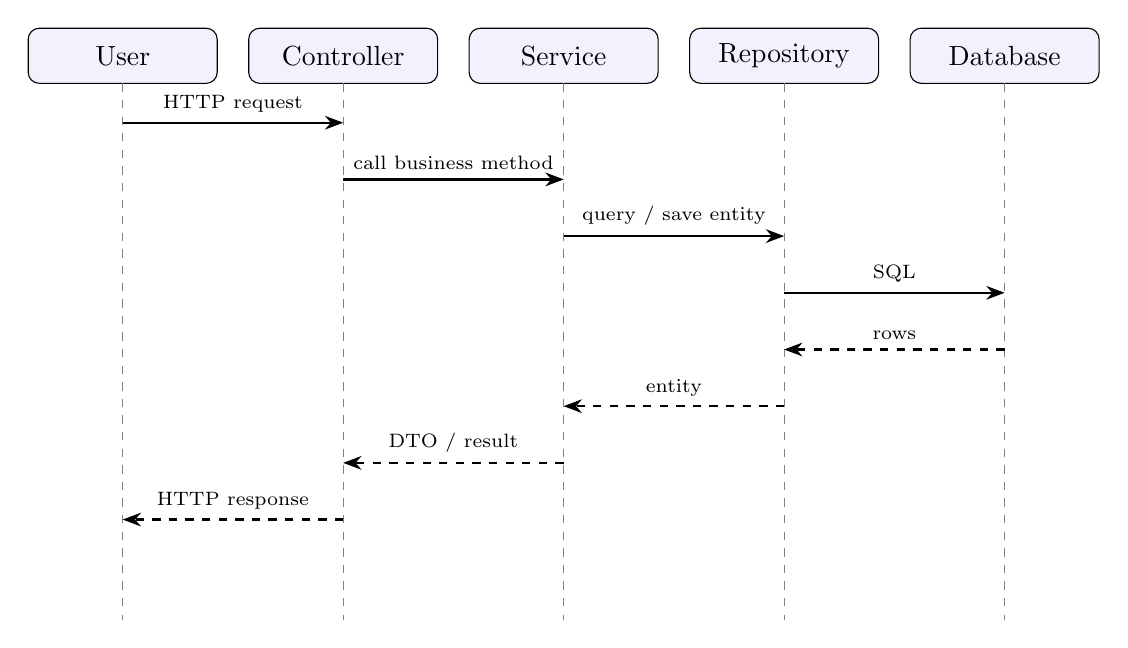
\begin{tikzpicture}[>=Stealth, lifeline/.style={dashed, gray}, head/.style={draw, rounded corners, fill=blue!5, align=center, minimum width=24mm, minimum height=7mm}, msg/.style={->, thick}, ret/.style={->, thick, dashed}]
\node[head] (p0) at (0.0,0) {User};
\draw[lifeline] (0.0,-0.35) -- (0.0,-7.16);
\node[head] (p1) at (2.8,0) {Controller};
\draw[lifeline] (2.8,-0.35) -- (2.8,-7.16);
\node[head] (p2) at (5.6,0) {Service};
\draw[lifeline] (5.6,-0.35) -- (5.6,-7.16);
\node[head] (p3) at (8.399999999999999,0) {Repository};
\draw[lifeline] (8.399999999999999,-0.35) -- (8.399999999999999,-7.16);
\node[head] (p4) at (11.2,0) {Database};
\draw[lifeline] (11.2,-0.35) -- (11.2,-7.16);
\draw[msg] (0.0,-0.85) -- node[above, font=\scriptsize, align=center] {HTTP request} (2.8,-0.85);
\draw[msg] (2.8,-1.57) -- node[above, font=\scriptsize, align=center] {call business method} (5.6,-1.57);
\draw[msg] (5.6,-2.29) -- node[above, font=\scriptsize, align=center] {query / save entity} (8.399999999999999,-2.29);
\draw[msg] (8.399999999999999,-3.01) -- node[above, font=\scriptsize, align=center] {SQL} (11.2,-3.01);
\draw[ret] (11.2,-3.73) -- node[above, font=\scriptsize, align=center] {rows} (8.399999999999999,-3.73);
\draw[ret] (8.399999999999999,-4.45) -- node[above, font=\scriptsize, align=center] {entity} (5.6,-4.45);
\draw[ret] (5.6,-5.17) -- node[above, font=\scriptsize, align=center] {DTO / result} (2.8,-5.17);
\draw[ret] (2.8,-5.89) -- node[above, font=\scriptsize, align=center] {HTTP response} (0.0,-5.89);
\end{tikzpicture}}
\end{center}



作图要点：Controller 只接收请求和返回响应；Service 处理业务逻辑；Repository 或 Mapper 访问数据库；箭头方向不能从 Repository 反向调用 Service。

题 3：画 JWT 登录流程。

\begin{center}
\resizebox{1.0\textwidth}{!}{%
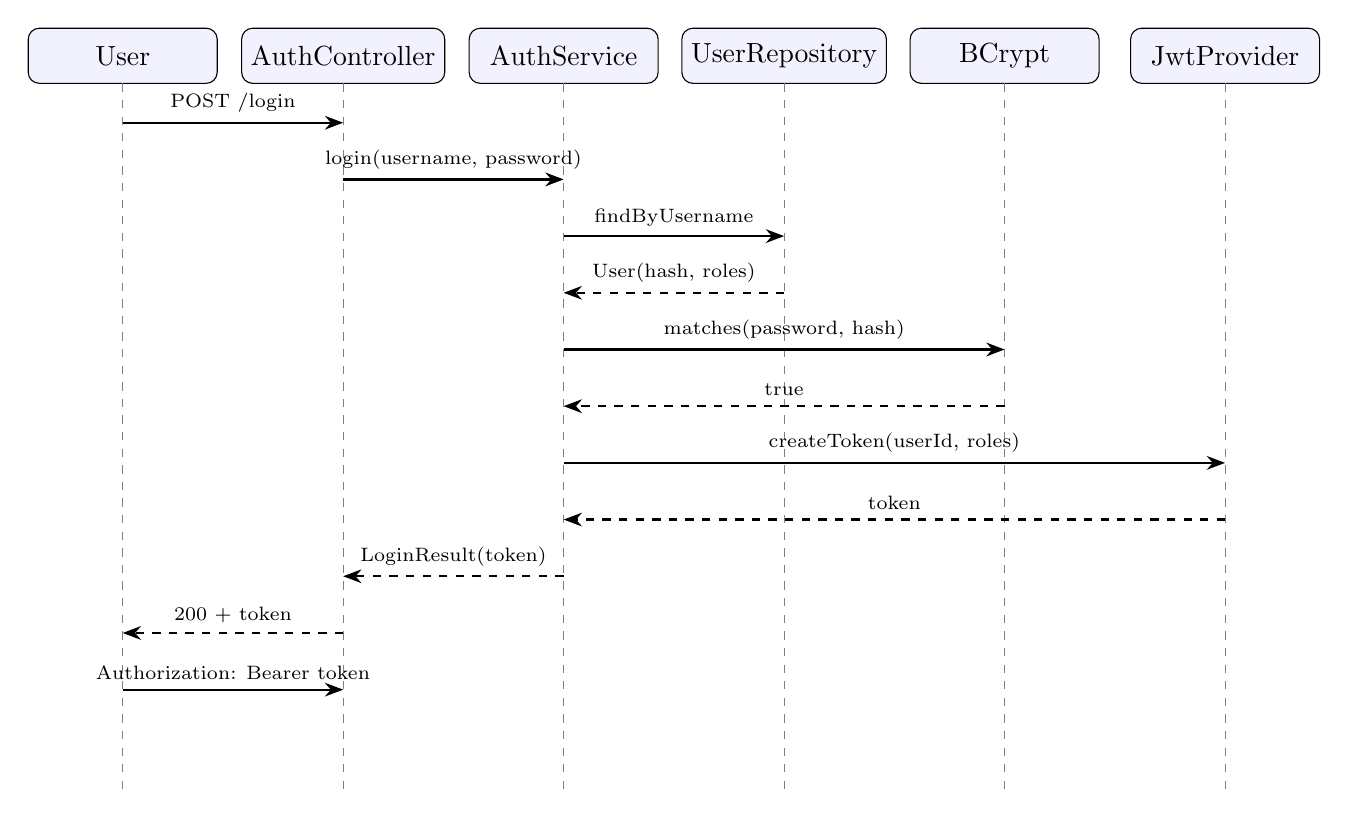
\begin{tikzpicture}[>=Stealth, lifeline/.style={dashed, gray}, head/.style={draw, rounded corners, fill=blue!5, align=center, minimum width=24mm, minimum height=7mm}, msg/.style={->, thick}, ret/.style={->, thick, dashed}]
\node[head] (p0) at (0.0,0) {User};
\draw[lifeline] (0.0,-0.35) -- (0.0,-9.32);
\node[head] (p1) at (2.8,0) {AuthController};
\draw[lifeline] (2.8,-0.35) -- (2.8,-9.32);
\node[head] (p2) at (5.6,0) {AuthService};
\draw[lifeline] (5.6,-0.35) -- (5.6,-9.32);
\node[head] (p3) at (8.399999999999999,0) {UserRepository};
\draw[lifeline] (8.399999999999999,-0.35) -- (8.399999999999999,-9.32);
\node[head] (p4) at (11.2,0) {BCrypt};
\draw[lifeline] (11.2,-0.35) -- (11.2,-9.32);
\node[head] (p5) at (14.0,0) {JwtProvider};
\draw[lifeline] (14.0,-0.35) -- (14.0,-9.32);
\draw[msg] (0.0,-0.85) -- node[above, font=\scriptsize, align=center] {POST /login} (2.8,-0.85);
\draw[msg] (2.8,-1.57) -- node[above, font=\scriptsize, align=center] {login(username, password)} (5.6,-1.57);
\draw[msg] (5.6,-2.29) -- node[above, font=\scriptsize, align=center] {findByUsername} (8.399999999999999,-2.29);
\draw[ret] (8.399999999999999,-3.01) -- node[above, font=\scriptsize, align=center] {User(hash, roles)} (5.6,-3.01);
\draw[msg] (5.6,-3.73) -- node[above, font=\scriptsize, align=center] {matches(password, hash)} (11.2,-3.73);
\draw[ret] (11.2,-4.45) -- node[above, font=\scriptsize, align=center] {true} (5.6,-4.45);
\draw[msg] (5.6,-5.17) -- node[above, font=\scriptsize, align=center] {createToken(userId, roles)} (14.0,-5.17);
\draw[ret] (14.0,-5.89) -- node[above, font=\scriptsize, align=center] {token} (5.6,-5.89);
\draw[ret] (5.6,-6.61) -- node[above, font=\scriptsize, align=center] {LoginResult(token)} (2.8,-6.61);
\draw[ret] (2.8,-7.33) -- node[above, font=\scriptsize, align=center] {200 + token} (0.0,-7.33);
\draw[msg] (0.0,-8.05) -- node[above, font=\scriptsize, align=center] {Authorization: Bearer token} (2.8,-8.05);
\end{tikzpicture}}
\end{center}



作图要点：JWT 只保存声明和权限信息，不保存密码；密码用 BCrypt 比对；后续请求通过 \texttt{Authorization: Bearer ...} 携带 Token。

\subsection{4. 代码分析题答案}

结合 \texttt{Exam/2022.pdf} 的 \texttt{doPost} 题型，分析 Web 后端代码时按下面结构答：

\begin{enumerate}
\item 可读性：参数命名要准确，方法长度要受控，条件表达式要拆分成有业务含义的布尔变量。
\item 模块化：Servlet 或 Controller 不应堆满业务规则，应把业务逻辑下沉到 Service，把数据访问下沉到 Repository 或 Mapper。
\item 异常路径：检查空值、非法参数、外部服务失败、数据库异常和重复提交。
\item 安全性：检查 SQL 注入、越权访问、敏感信息泄露、密码明文处理和 CSRF 风险。
\item 资源管理：数据库连接、文件流和网络连接要被正确关闭，事务要能回滚。
\item 测试覆盖：至少覆盖正常路径、边界条件、非法输入、异常路径和权限失败。
\end{enumerate}

\section{十二、最后复习抓手}

00 部分可以用一条线串起来：

\begin{quote}
\footnotesize
\begin{verbatim}
AI 协作意识
→ Prompt / Spec
→ Git / DevOps 留痕和交付
→ 前端 HTML/CSS/JS + Vue
→ 后端 HTTP/REST/JSON + Spring Boot
→ 数据 MyBatis + 安全 Spring Security/JWT
→ VibeCoding 全链路生成、调试、联调
→ 人负责审查、测试、安全和工程决策
\end{verbatim}
\end{quote}

最容易和旧考点结合的部分：

\begin{itemize}
\item 2020：Web 分层、REST、客户端/服务器端划分。
\item 2022：Servlet / \texttt{doPost}、代码构造质量、测试覆盖。
\item 2025：AI 语境、SpringBoot 三层职责、接口声明、依赖注入、三层顺序图。
\end{itemize}

最不能忽略的答题原则：

\begin{itemize}
\item 不要把 AI 当作责任主体。
\item 不要把登录、数据检查、连接数据库、网络传输写成业务用例。
\item 不要混淆 \texttt{Controller}、\texttt{Service}、\texttt{Repository}、\texttt{Mapper}。题目给什么标识符，就使用什么标识符。
\item 不要把 \texttt{\#\{\}} 和 \texttt{\$\{\}} 混用。
\item 不要把 JWT Payload 当作加密存储。
\item 不要只写工具名，要写工具在工程流程中的作用。
\end{itemize}
\end{document}

